\documentclass[fr]{../../../../../../eplexam}

\newcommand*\Eval[3]{\left.#1\right\rvert_{#2}^{#3}}

\hypertitle{Signaux et systèmes}{4}{FSAB}{1106}{2014}{Juin}{All}
{Louis Devillez \and Gilles Peiffer}
{Luc Vandendorpe et Vincent Wertz}

\section{Question VW1}
On considère le système causal représenté à la figure suivante:
\begin{center}
	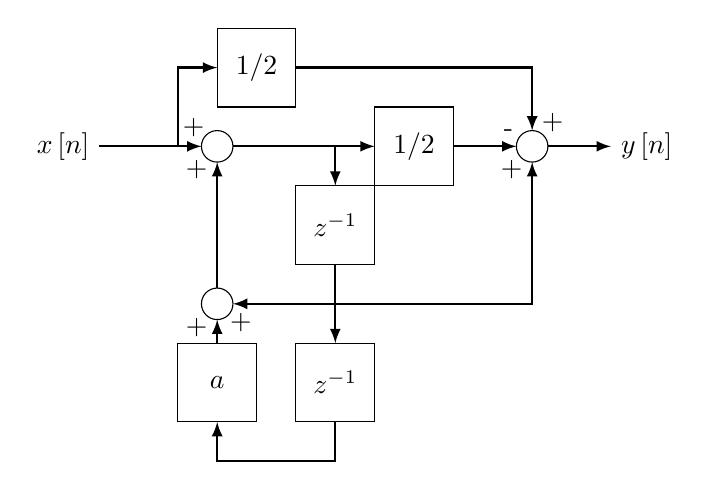
\begin{tikzpicture}
		\draw (-0.5,0) node[left]{$x\left[n\right]$} [thick,-latex] --(0.8,0);
		\draw (0.7,0)node[above]{+};
		\draw (1,0) circle(0.2);
		\draw [thick,-latex] (0.5,0) -- (0.5,1) -- (1,1);
		\draw (1,1.5) rectangle (2,0.5);
		\draw (1.5,1) node[]{1/2};
		\draw [thick,-latex](1.2,0) -- (2.5,0) -- (2.5,-0.5);
		\draw [thick,-latex](2.5,0) -- (3,0);
		\draw (3,0.5) rectangle (4,-0.5);
		\draw (3.5,0)node[]{1/2};
		\draw [thick,-latex](4,0) --(4.8,0);
		\draw (4.7,0)node[above]{-};
		\draw [thick,-latex] (2,1) -- (5,1) -- (5,0.2);
		\draw (5,0.3)node[right]{+};
		\draw (5,0) circle(0.2);
		\draw (2,-0.5) rectangle (3,-1.5);
		\draw (2.5,-1)node[]{$z^{-1}$};
		\draw [thick,-latex](2.5,-1.5) -- (2.5,-2) -- (1.2,-2);
		\draw (1.3,-2)node[below]{+};
		\draw (1,-2) circle(0.2);
		\draw [thick,-latex] (1,-1.8) -- (1,-0.2);
		\draw (1,-0.3) node[left]{+};
		\draw [thick,-latex] (2.5,-2) -- (2.5,-2.5);
		\draw (2,-2.5) rectangle (3,-3.5);
		\draw (2.5,-3) node[]{$z^{-1}$};
		\draw [thick,-latex] (2.5,-3.5) -- (2.5,-4) -- (1,-4) -- (1,-3.5);
		\draw (0.5,-3.5) rectangle (1.5,-2.5);
		\draw (1,-3) node[]{$a$};
		\draw [thick,-latex](1,-2.5) -- (1,-2.2);
		\draw (1,-2.3) node[left]{+};
		\draw [thick,-latex](2.5,-2) -- (5,-2) -- (5,-0.2);
		\draw (5,-0.3)node[left]{+};
		\draw [thick,-latex] (5.2,0) -- (6,0)node[right]{$y\left[n\right]$};
	\end{tikzpicture}
\end{center}
\begin{itemize}
	\item Déterminer une représentation d'état du système.
	\item Calculer la fonction de transfert associée.
	\item Étudier la stabilité interne du système pour les mêmes valeurs du paramètre $a=0$, $a=1$ et $a=2$.
	\item Étudiez la stabilité BIBO/EBSB du système pour les mêmes valeurs du paramètre $a$.
	\item Définir en quelques lignes la notion de commandabilité d'un système linéaire.
	\item Étudiez la commandabilité et l'observabilité du système pour les trois valeurs du paramètre $a$ mentionnées plus haut.
\end{itemize}

\begin{solution}
	\begin{itemize}
		\item Représentation d'état:	$$
		\begin{pmatrix}
		q_1\left[n+1\right]\\
		q_2\left[n+1\right]
		\end{pmatrix}=
		\begin{pmatrix}
		1&a\\
		1&0
		\end{pmatrix}
		\begin{pmatrix}
		q_1\left[n\right]\\
		q_2\left[n\right]
		\end{pmatrix}
		+
		\begin{pmatrix}
		1\\
		0
		\end{pmatrix}
		x\left[n\right]$$
		$$
		y\left[n\right]=
		\begin{pmatrix}
		1/2 & -a/2
		\end{pmatrix}
		\begin{pmatrix}
		q_1\left[n\right]\\
		q_2\left[n\right]
		\end{pmatrix}
		+
		\begin{pmatrix}
		0
		\end{pmatrix}
		x\left[n\right].$$

		\item Fonction de transfert :
		\begin{align*}
			H(z) &= C(zI-A)^{-1}B + D\\ &= \cfrac{z-a}{2(z^2-z-a)}.
		\end{align*}

		\item Stabilité interne :

		La matrice $A$ est

		\begin{equation*}
			A = \begin{pmatrix}
			1&a\\
			1&0
			\end{pmatrix}.
		\end{equation*}

		Son polynôme caractéristique vaut

		\begin{align*}
			P(\lambda) &= \det(A - \lambda I)\\
			&= (1 - \lambda) (-\lambda) - a\\
			&= \lambda^2 - \lambda - a.
		\end{align*}

		\begin{itemize}
		\item Soit $a = 0$

		\begin{align*}
			P(\lambda) = \lambda^2 - \lambda.
		\end{align*}

		Les valeurs propres de $A$ (c'est-à-dire les racines de $P(\lambda)$) sont $\lambda_1 = 0$ et $\lambda_2 = 1$.
		On voit que $\abs{\lambda_i} \leq 1$; le système est marginalement stable.


		\item Soit $a = 1$

		\begin{align*}
			P(\lambda) = \lambda^2 - \lambda - 1.
		\end{align*}

		Les valeurs propres de $A$ (c'est-à-dire les racines de $P(\lambda)$) sont $\lambda_1 = \cfrac{1 + \sqrt{5}}{2}$
		et $\lambda_2 = \cfrac{1 - \sqrt{5}}{2}$.
		On voit que $\abs{\lambda_1} > 1$; le système est instable.


		\item Soit $a = 2$

		\begin{align*}
			P(\lambda) = \lambda^2 - \lambda - 2.
		\end{align*}

		Les valeurs propres de $A$ (c'est-à-dire les racines de $P(\lambda)$) sont $\lambda_1 = 2$
		et $\lambda_2 = -1$.
		On voit que $\abs{\lambda_1} > 1$; le système est instable.
		\end{itemize}

		\item La fonction de transfert vaut en toute généralité

		\begin{align*}
			H(z) = \cfrac{z-a}{2(z^2-z-a)}.
		\end{align*}
		\begin{itemize}
		\item Soit $a = 0$

		La fonction de transfert devient alors

		\begin{align*}
			H(z) &= \cfrac{z-a}{2(z^2-z-a)}\\
			&= \cfrac{z}{2z(z-1)}\\
			&= \cfrac{1}{2(z-1)}.
		\end{align*}

		Il y a un pôle $p_1$ en $z = 1$.
		Comme $\abs{p_1} \geq 1$, le système est BIBO/EBSB instable.

		\item Soit $a = 1$

		La fonction de transfert devient alors

		\begin{align*}
			H(z) &= \cfrac{z-a}{2(z^2-z-a)}\\
			&= \cfrac{z - 1}{2(z^2 - z - 1)}.
		\end{align*}

		Il y a deux pôles, $p_1$ et $p_2$, en $z = \cfrac{1 + \sqrt{5}}{2}$
		et $z = \cfrac{1 - \sqrt{5}}{2}$.
		Comme $\abs{p_1} \geq 1$, le système est BIBO/EBSB instable.

		\item Soit $a = 2$

		La fonction de transfert devient alors

		\begin{align*}
			H(z) &= \cfrac{z-a}{2(z^2-z-a)}\\
			&= \cfrac{z - 2}{2(z^2 - z - 2)}\\
			&= \cfrac{1}{2(z + 1)}.
		\end{align*}

		Il y a un pôle $p_1$ en $z = -1$. Comme $\abs{p_1} \geq 1$, le système est BIBO/EBSB instable.
		\end{itemize}

		\item Soit $\mathcal{Q}$ l'espace d'état (l'ensemble des valeurs que peut prendre $q(t)$).
		Un système est dit commandable si pour tout intervalle de temps
		$[t_{\textnormal{i}}, t_{\textnormal{f}}]$, et tous points
		$q_{\textnormal{i}}, q_{\textnormal{f}} \in \mathcal{Q}$,
		avec $q(t_{\textnormal{i}}) = q_{\textnormal{i}}$,
		il existe une commande $u$ (une suite d'entrées)
		appliquée sur $[t_{\textnormal{i}}, t_{\textnormal{f}}]$,
		telle que $q(t_{\textnormal{f}}) = q_{\textnormal{f}}$.

		En français : un système est dit commandable si on peut partir de
		n'importe quel état de départ et arriver à n'importe quel état d'arrivée
		en un temps fini.

		Un système est donc commandable si tous ses états le sont aussi.
		\item Commandabilité et observabilité

		\begin{align*}
			\mathcal{C}(A, B) &= \begin{pmatrix}
		B & AB
		\end{pmatrix}\\
		&= \begin{pmatrix}
		1 & 1\\
		0 & 1
		\end{pmatrix}.
		\end{align*}

		Cette matrice est toujours de plein rang (ses colonnes sont linéairement indépendantes)
		et le système est donc toujours complètement commandable peu importe la valeur de $a$.

		\begin{align*}
			\mathcal{O}(A, C) &= \begin{pmatrix}
		C\\
		CA
		\end{pmatrix}\\
		&= \begin{pmatrix}
		1/2 & -a/2\\
		1/2 - a/2 & a/2
		\end{pmatrix}.
		\end{align*}

		Lorsque $a = 0$ ou $a = 2$, cette matrice n'est pas de plein rang
		et le système n'est donc pas complètement observable.
		Cependant, lorsque $a = 1$, il l'est.

		On pouvait s'attendre à voir une perte soit de commandabilité soit d'observabilité
		car on a vu que dans les cas $a = 0$ et $a = 2$ on avait une annulation pôle/zéro.

	\end{itemize}
\end{solution}

\section{Question VW2}
On considère un système continu LTI décrit par l'équation différentielle suivante:
$$y''(t) - y'(t) -6y(t) = x(t) +x'(t).$$
\begin{itemize}
	\item Calculer la fonction de transfert du système.
	\item Déterminer la réponse impulsionnelle du système dans chacun des cas suivants:
	\subitem le système est causal;
	\subitem le système est stable au sens BIBO/EBSB.
	\item Esquisser sommairement la réponse impulsionnelle dans chacun des deux cas.
	\item Pour le cas BIBO/EBSB stable, calculer la sortie du système correspondant à l'entrée $x(t) = \e^{-t}$. Commenter le résultat obtenu (indication: réfléchir et/ou utiliser le produit de convolution).
\end{itemize}

\begin{solution}
	\begin{itemize}
		\item Fonction de transfert.
	\begin{align*}
		H(s) = \frac{Y(s)}{X(s)}.
	\end{align*}
	L'équation différentielle devient
	\begin{align*}
		s^2 Y(s) - sY(s) - 6Y(s) &= X(s) + sX(s).
	\end{align*}

	On trouve donc

	\begin{align*}
		H(s) &= \frac{s + 1}{s^2 - s - 6}\\
		&= \frac{s + 1}{(s - 3)(s + 2)}.
	\end{align*}

	\item Réponse impulsionnelle.

	En faisant une décomposition en fractions simples :

	\begin{align*}
		H(s) &= \frac{s + 1}{(s - 3)(s + 2)}\\
		&= \frac{\alpha}{(s - 3)} + \frac{\beta}{(s + 2)}\\
		&= \frac{\frac{4}{5}}{(s - 3)} + \frac{\frac{1}{5}}{(s + 2)}.
	\end{align*}

	\begin{itemize}
		\item Système causal.

		Si le système est causal, la $\mathrm{ROC}$ est un demi-plan à droite
		d'un certain axe vertical. Cette $\mathrm{ROC}$ ne contient
		pas de pôles et le demi-plan doit donc être
		le demi-plan à droite de $\Re\{s\} = 3$.
		On trouve alors dans les tables que
	$$h(t) = \frac{1}{5} \left(4 \e^{3t} + \e^{-2t} \right) u(t).$$
	\begin{center}
		\begin{tikzpicture}
			\draw [thick,-latex] (-4,0) --(4,0);
			\draw [thick,-latex] (0,-0.5) -- (0,2);
			\draw [domain=0:0.5,samples=200] plot(\x,{4/5*exp(\x*3)+1/5*exp(\x *-2)});
		\end{tikzpicture}
	\end{center}
	\item Système BIBO/EBSB stable.

	Si le système est BIBO/EBSB stable, l'axe imaginaire doit être
	dans la $\mathrm{ROC}$.
	Celle-ci étant l'intersection des $\mathrm{ROC}$ des deux fractions simples,
	il faut prendre pour $\mathrm{ROC}$ l'intersection de $\Re\{s\} < 3$
	pour le terme avec $s - 3$ et
	$\Re\{s\} > -2$ pour le terme avec $s + 2$. On trouve alors
	$$h(t) = \frac{1}{5} \left(\e^{-2t} u(t) - 4 \e^{3t} u(-t) \right).$$
	\begin{center}
		\begin{tikzpicture}
		\draw [thick,-latex] (-4,0) --(4,0);
		\draw [thick,-latex] (0,-1.5) -- (0,2);
		\draw [domain=0:4,samples=200] plot(\x,{1/5*exp(\x *-2)});
		\draw [domain=-4:0,samples=200] plot(\x,{-4/5*exp(\x * 3)});
		\end{tikzpicture}
	\end{center}
	\end{itemize}
	\item La fonction de transfert a un zéro en $s=1$. La sortie du système correspondant à une entrée
	$x(t) = \e^{at}$ est $y(t) = H(a) x(t)$. Le raisonnement pour ceci est que $\e^{at}$
	est une ``fonction propre'' avec comme ``valeur propre'' associée $H(a)$.
	Ici, cela permet de déduire que
	\begin{align*}
		y(t) &= H(-1) \e^{-t}\\
		&= 0.
	\end{align*}

	Alternativement, on peut passer par le produit de convolution.

	\begin{align*}
		y(t) &= \int_{-\infty}^{+\infty} \left( \frac{1}{5} \e^{-2\tau} u(\tau) - \frac{4}{5} \e^{3\tau} u(-\tau)\right) \e^{-(t -\tau)} \dif{\tau}\\
		&= \e^{-t} \left( \int_{-\infty}^{0} -\frac{4}{5} \e^{4 \tau} \dif{\tau} +  \int_{0}^{+\infty} \frac{1}{5} \e^{- \tau} \dif{\tau} \right)\\
		&= \e^{-t} \left( \Eval{-\frac{1}{5} \e^{4 \tau}}{-\infty}{0} - \Eval{\frac{1}{5} \e^{- \tau}}{0}{+\infty} \right)\\
		&= \e^{-t} \left( -\frac{1}{5} + \frac{1}{5} \right)\\
		&= 0.
	\end{align*}

	C'est évidemment la même chose qu'avec la première méthode.
	\end{itemize}
\end{solution}
\end{document}
